\chapter{Experimental Results} \label{ch:ExperimentalResults}
In this Chapter we will cover the experimental phase of our work. First comes a description of our setup and methodology, covering the hardware and software utilized as well as the chosen benchmarks and metrics. Then we will present our results and provide our analysis in order to fuel further research and development in the MANGO software stack.

Our main goals during this experimental campaign were:
\begin{itemize}
    \item Measure the performance of MANGO with respect to other available programming models.
    \item Compare the programmability of MANGO with respect to other available programming models.
    \item Analyze where are the main overheads of the current MANGO implementation and how they can be reduced.
\end{itemize}

\section{Setup and Methodology}
All our tests were run on a Dell XPS 9570 laptop. This particular model is equipped with an Intel Core i7 8750H CPU, 16 GB RAM and an NVIDIA GeForce GTX 1050 Ti with Max-Q Design GPU (4GB VRAM). In terms of Operating System, the machine was running Ubuntu 18.04.2 LTS 64-bit (Kernel Version: 5.4.0-48-generic).

For reproducibility, the versions of the software run are as follows:
\begin{itemize}
    \item CUDA 11.0
    \item OpenCL 1.2 CUDA (Driver version: 450.51.06)
    \item gcc 7.5.0 (Ubuntu 7.5.0-3ubuntu1~18.04)
    \item clang 6.0.0-1ubuntu2
    \item Python 3.6.9
    \item Cython 0.29.23
\end{itemize}

In order to compare the performance of MANGO to CUDA and OpenCL we used a subset of the Rodinia Benchmark Suite (Version 3.1) \cite{rodinia}, provided by the University of Virginia. In particular, we chose the HotSpot and PathFinder benchmarks.

HotSpot (HS) is a thermal simulation tool, presented in \cite{hotspot}, which is used for estimating processor temperature based on an architectural floor plan and simulated power measurements. The benchmark includes the 2D transient thermal simulation kernel of HotSpot, which iteratively solves a series of differential equations for block temperatures. The inputs to the program are power and initial temperatures of a square N x N grid. Each output cell in the grid represents the average temperature value of the corresponding area of the chip.

During our experiments, the size of the Grid (N) was progressively increased in order to increase the load on the GPU. The number of threads spawned for computation as well as the size of the input buffers and output buffers scale with O(N\textsuperscript{2}). The number of kernel executions is determined by the amount of iterations desired. This parameter is kept fixed, resulting in 16 kernel executions to compute 128 iterations of the algorithm for all HotSpot benchmarks.

PathFinder (PF) uses dynamic programming to find a path on a 2-D grid from the bottom row to the top row with the smallest accumulated weights, where each step of the path moves straight ahead or diagonally ahead. It iterates row by row, each node picks a neighboring node in the previous row that has the smallest accumulated weight, and adds its own weight to the sum.

Like with HotSpot, we also increased the size of the input grid (N) in order to increase the GPU load when running the PathFinder benchmarks. The dimensions of the grid were also kept symmetrical, as in the number of columns is equal to the number of rows (N x N). In this case, increasing the number of columns increases the number of threads spawn to compute the shortest path. The number of rows, on the other hand, increases the number of kernel executions. In addition, the size of the grid increases the dimensions of the input buffer with O(N\textsuperscript{2}), the output however only increases linearly, with O(N), as only the values of the columns are needed.

During our testing we realized that PathFinder most certainly lacks global GPU memory access optimizations. This is indicated by its poor memory bandwidth performance coupled with the fact that the algorithm requires constant access to the input rows in order to calculate each iteration. In addition, the operations performed by pathfinder are simple comparisons and a single integer addition. It is important to also note that these comparisons are integer minimum operations, which do not generate branches \cite{ptx_isa}.

We still decided to keep PathFinder in our comparison as it is a good example of what happens when there is a need to run a kernel multiple times in a single benchmark and how the different systems scale with increasing numbers of kernel launches.

Finally, in order to cover our lack of memory bound applications due to the issues mentioned with PathFinder, we added an AXPY benchmark. AXPY stands for "A X plus Y", as noted by the name, it performs the following operation:

\[
    z \leftarrow a*x+y
\]

This same operation is also implemented in BabelStream \cite{babelstream}, a memory bandwidth benchmark for heterogenous systems based on STREAM \cite{stream}, which names it "Triad". 

A breakdown of the three benchmarks chosen can be seen in table \ref{tab:benchmark-breakdown}.

\begin{table}[ht]
    \centering
    \begin{tabular}{l|c|c}
    Benchmark & Dwarves & Performance characteristic \\ \hline
    HotSpot & Structured Grid & Compute intensive \\
    PathFinder & Dynamic Programming & Multiple kernel launches \\
    AXPY & Basic Linear Algebra & Memory intensive          
    \end{tabular}
    \captionsetup{justification=centering}
    \caption{Breakdown of benchmarks used}
    \label{tab:benchmark-breakdown}
\end{table}

\subsection{Performance metrics}

To evaluate performance in both HotSpot and PathFinder, we will measure:

\begin{itemize}
    \item Total execution time: time since the beginning of the proper benchmark (i.e. after all input initialization and I/O) and the end (after all resource deallocations, but before checking output results).
    \item Kernel execution time: time since the launch of a kernel and the end of its execution.
    \item Buffer write time: time to write data to the device, i.e transfer data from the host to the device.
    \item Buffer read time: time to read data from the device, i.e. transfer data from the device to the host.
\end{itemize}

For AXPY, we will measure the performance of the different systems as the percentage of theoretical peak bandwidth they can achieve. We will take into account both GPU memory bandwidth, measuring accesses to GPU global memory, and PCI-E bandwidth, measuring data transfers between the Host and the Device and vice versa.

For GPU memory, the theoretical peak bandwidth is given by plugging the memory clock rate and bus width into the following formula:

\[
    GBW_{peak} = \frac{C * 10^6 * (B/8) * 2}{10^9}
\]

Where:
\begin{itemize}
    \item $GBW_{peak}$ is the theoretical peak GPU VRAM bandwidth in GB/s.
    \item $C$ is the memory clock rate in MHz.
    \item $B$ is the memory bus width in bits.
\end{itemize}

With a memory clock rate of 3504 MHz and 128-bit of bus width, the GTX 1050 Ti in our test bench achieves a theoretical peak of 112.128 GB/s.

To measure the effective bandwidth achieved by each model we use the following formula:

\[
    GBW_{effective} = \frac{R_B + W_B}{t * 10^9}
\]

Where:
\begin{itemize}
    \item $GBW_{effective}$ is the effective GPU VRAM bandwidth in GB/s.
    \item $R_B$ is the number of bytes read per kernel.
    \item $W_B$ is the number of bytes written per kernel.
    \item $t$ is the kernel execution time in seconds.
\end{itemize}

The two previous formulae were taken from \cite{perf_metrics_cuda}.

In terms of PCI-E bandwidth, our video card presents a PCI-E 3.0 x16 connection which could achieve a peak bandwidth of 15.754GB/s.

In a very similar way as how we measure effective bandwidth for GPU memory, we can measure the effective transfer bandwidth:

\[
    TBW_{effective} = \frac{T_B}{t * 10^9}
\]

Where:
\begin{itemize}
    \item $TBW_{effective}$ is the effective transfer bandwidth in GB/s.
    \item $T_B$ is the number of bytes transferred.
    \item $t$ is the transfer time in seconds.
\end{itemize}

In AXPY we are not interested in the scaling over different input sizes but in the bandwidths achieved with large inputs. A large input maximizes the amount of memory to transfer and access, meaning that a larger part of the available bandwidth can be exploited.  

Finally, it is important to note that for all benchmarks in both CUDA and OpenCL we execute the set of benchmarks twice. Once to measure the total execution time of the entire benchmark and another to measure each individual component. As all our measurements in these models are done externally (i.e. we cannot make intrusive profiling modifications like with MANGO) they could incur in extra overhead due to the need of forcing synchronization between the host and the device in order to make measurements. For example, OpenCL buffer writes are usually enqueued in a \texttt{CommandQueue} and executed asynchronously, to measure them we forced a synchronous transfer by calling \texttt{clFinish} on the \texttt{CommandQueue}.

\subsection{Programmability}

To compare the programmability of each model we count the number of lines of code (LOC) required for each implementation of the HotSpot and PathFinder benchmarks. To compute the LOC we do not take into account comments or blank lines. Also, we ignore any line of code related to debugging, extra code needed to profile the OpenCL and CUDA benchmarks or checking computation results. This last point is particularly significant on the MANGO benchmarks which usually compare their results with the CUDA benchmarks to ensure that the implementation is working correctly. Finally, the original code from the Rodinia Benchmarks was adapted in order to follow a consistent style across all implementations. 

In addition to the LOC metric, to have a more direct comparison of the size of the MANGO implementations to the CUDA and OpenCL ones we also use a Relative Difference metric (RD). RD calculates the percentage difference in LOC between MANGO and a different implementation. We define RD as follows:

\[
    RD = \frac{LOC_{impl} - LOC_{MANGO}}{LOC_{MANGO}} * 100
\]

Thus, a positive RD indicates that a given implementation requires more LOC than MANGO, while a negative RD indicates that the implementation requires less LOC.

\section{Results}

In this section we will present the results of our experiments results and provide an analysis of our implementation's strengths and weaknesses.

\subsection{Performance}

\subsubsection{HotSpot}

Starting with HotSpot, we can see a clear, but not excessively large, difference in performance between our MANGO and the other two models by looking at the mean total execution time in figure \ref{fig:hotspot_total_duration_mean}. This difference becomes larger as the input size increases, which points towards the majority of the overhead being present in the memory transfers.

\begin{figure}[ht]
    \centering
    \resizebox{0.6\textwidth}{!}{
        % This file was created by tikzplotlib v0.9.8.
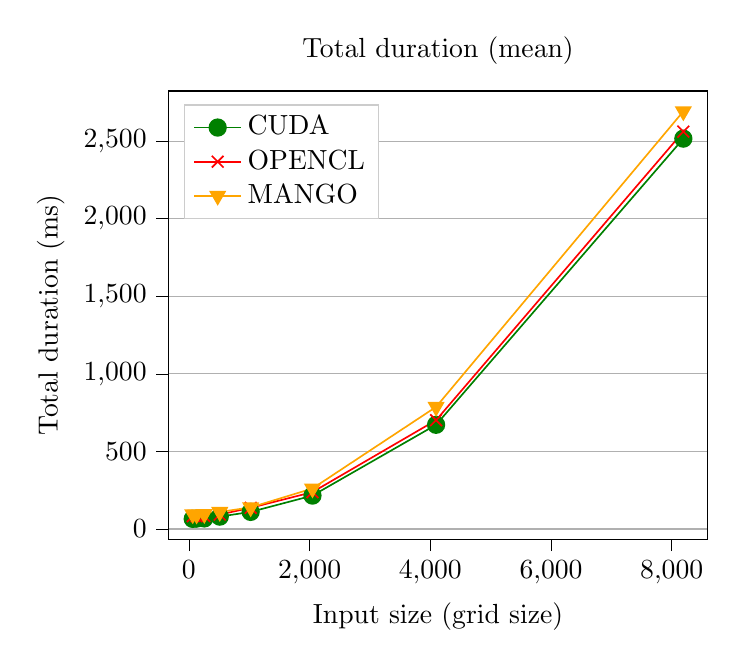
\begin{tikzpicture}

\definecolor{color0}{rgb}{1,0.647058823529412,0}

\begin{axis}[
legend cell align={left},
legend style={
  fill opacity=1,
  draw opacity=1,
  text opacity=1,
  at={(0.03,0.97)},
  anchor=north west,
  draw=white!80!black
},
tick align=outside,
tick pos=left,
title={Total duration (mean)},
x grid style={white!69.0196078431373!black},
xlabel={Input size (grid size)},
xmin=-342.4, xmax=8598.4,
xtick style={color=black},
y grid style={white!69.0196078431373!black},
ylabel={Total duration (ms)},
ymajorgrids,
ymin=-65.959002829394, ymax=2823.53145097283,
ytick style={color=black}
]
\addplot [semithick, green!50.1960784313725!black, mark=*, mark size=3, mark options={solid}]
table {%
64 65.3814723434343
128 67.1212662244898
256 68.3322663666667
512 80.0275030333333
1024 110.4768081
2048 215.540796947368
4096 671.9512696
8192 2516.1915956
};
\addlegendentry{CUDA}
\addplot [semithick, red, mark=x, mark size=3, mark options={solid}]
table {%
64 82.7704575208333
128 82.79732128
256 83.8056829333333
512 93.437536862069
1024 136.60162595
2048 237.940542842105
4096 701.5180952
8192 2561.3243602
};
\addlegendentry{OPENCL}
\addplot [semithick, color0, mark=triangle*, mark size=3, mark options={solid,rotate=180}]
table {%
64 95.13603588
128 93.41098096
256 96.4721031
512 110.236007833333
1024 139.4998439
2048 261.1760106
4096 787.2880039
8192 2692.1909758
};
\addlegendentry{MANGO}
\end{axis}

\end{tikzpicture}

    }
    \captionsetup{justification=centering}
    \caption{Mean total execution time for HotSpot}
    \label{fig:hotspot_total_duration_mean}
\end{figure}

This is confirmed by figure \ref{fig:hotspot_kernel_executions_mean} which shows the kernel execution time for each model, although an overhead is present, it does not scale with the input size. This makes sense as the underlying kernel implementation is written in CUDA and compiled offline with NVIDIA's own NVRTC \cite{nvrtc}.

\begin{figure}[ht]
    \centering
    \resizebox{0.6\textwidth}{!}{
        % This file was created by tikzplotlib v0.9.8.
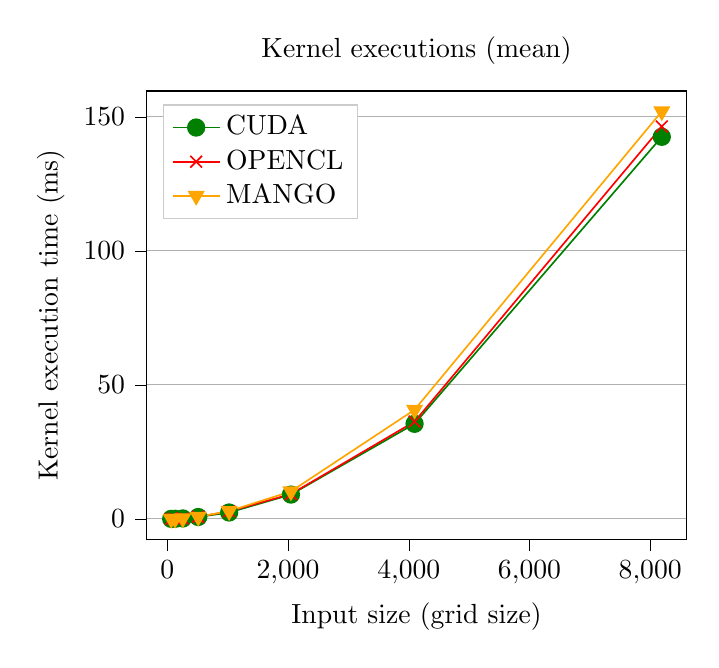
\begin{tikzpicture}

\definecolor{color0}{rgb}{1,0.647058823529412,0}

\begin{axis}[
legend cell align={left},
legend style={
  fill opacity=1,
  draw opacity=1,
  text opacity=1,
  at={(0.03,0.97)},
  anchor=north west,
  draw=white!80!black
},
tick align=outside,
tick pos=left,
title={Kernel executions (mean)},
x grid style={white!69.0196078431373!black},
xlabel={Input size (grid size)},
xmin=-342.4, xmax=8598.4,
xtick style={color=black},
y grid style={white!69.0196078431373!black},
ylabel={Kernel execution time (ms)},
ymajorgrids,
ymin=-7.58184667491691, ymax=159.663488779392,
ytick style={color=black}
]
\addplot [semithick, green!50.1960784313725!black, mark=*, mark size=3, mark options={solid}]
table {%
64 0.0202140275516594
128 0.0516223956466069
256 0.184729111111111
512 0.725393121412804
1024 2.39956375632911
2048 9.09626238291139
4096 35.4947399367089
8192 142.560531045161
};
\addlegendentry{CUDA}
\addplot [semithick, red, mark=x, mark size=3, mark options={solid}]
table {%
64 0.0204119285237141
128 0.0538414779706275
256 0.190541695364238
512 0.780070042826552
1024 2.83085394321767
2048 9.27893204444444
4096 36.3103518152866
8192 146.39821255625
};
\addlegendentry{OPENCL}
\addplot [semithick, color0, mark=triangle*, mark size=3, mark options={solid,rotate=180}]
table {%
64 0.0414139624681934
128 0.0703628888888889
256 0.211658812903226
512 0.81808229004329
1024 2.9290935968254
2048 10.27900955
4096 40.7308336708861
8192 152.061428076923
};
\addlegendentry{MANGO}
\end{axis}

\end{tikzpicture}

    }
    \captionsetup{justification=centering}
    \caption{Mean kernel execution time for HotSpot}
    \label{fig:hotspot_kernel_executions_mean}
\end{figure}

If we shift our focus over to buffer writes and reads which are shown in figure \ref{fig:hotspot_buffer_transfers_mean} respectively we can see that the source of the overhead is present here. MANGO memory transfers scale linearly with the size of the buffer as expected, but in a much steeper way compared to CUDA and OpenCL.

\begin{figure}[ht]%
    \centering
    \subfloat[\centering Mean buffer write time]{{
        \resizebox{0.45\textwidth}{!}{
        % This file was created by tikzplotlib v0.9.8.
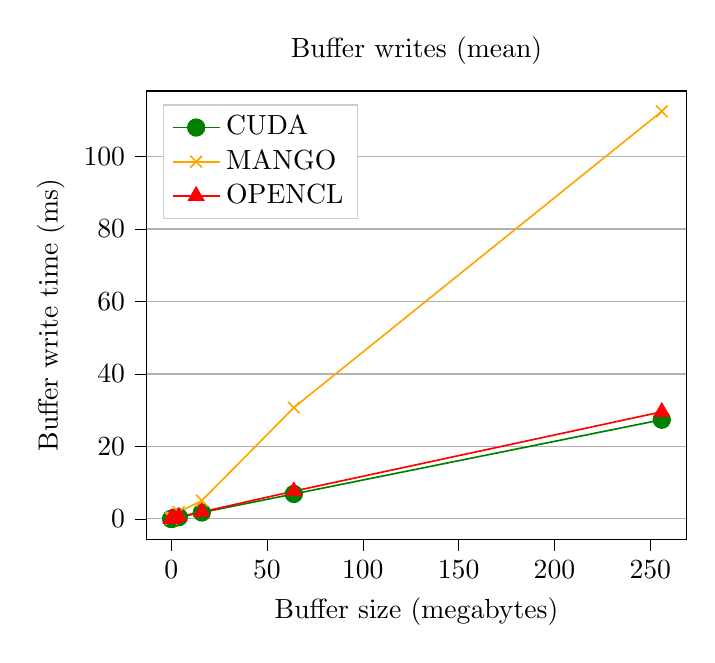
\begin{tikzpicture}

\definecolor{color0}{rgb}{1,0.647058823529412,0}

\begin{axis}[
legend cell align={left},
legend style={
  fill opacity=1,
  draw opacity=1,
  text opacity=1,
  at={(0.03,0.97)},
  anchor=north west,
  draw=white!80!black
},
tick align=outside,
tick pos=left,
title={Buffer writes (mean)},
x grid style={white!69.0196078431373!black},
xlabel={Buffer size (megabytes)},
xmin=-12.78359375, xmax=268.79921875,
xtick style={color=black},
y grid style={white!69.0196078431373!black},
ylabel={Buffer write time (ms)},
ymajorgrids,
ymin=-5.6126042730303, ymax=118.094086289192,
ytick style={color=black},
yticklabel style={/pgf/number format/fixed},
]
\addplot [semithick, green!50.1960784313725!black, mark=*, mark size=3, mark options={solid}]
table {%
0.015625 0.0104271161616162
0.0625 0.0190681313131313
0.25 0.0421460666666667
1 0.138006
4 0.479187025
16 1.777260975
64 6.89048626315789
256 27.3749119473684
};
\addlegendentry{CUDA}
\addplot [semithick, color0, mark=x, mark size=3, mark options={solid}]
table {%
0.015625 0.132945717948718
0.0625 0.1841103
0.25 0.203108508474576
1 0.371122457627119
4 1.873227375
16 5.05497213157895
64 30.71298635
256 112.4710549
};
\addlegendentry{MANGO}
\addplot [semithick, red, mark=triangle*, mark size=3, mark options={solid}]
table {%
0.015625 0.0693875846153846
0.0625 0.0795439081632653
0.25 0.1081564
1 0.245969101694915
4 0.625349487179487
16 1.934185
64 7.6582627
256 29.54956935
};
\addlegendentry{OPENCL}
\end{axis}

\end{tikzpicture}

    } 
    }}%
    \qquad
    \subfloat[\centering Mean buffer read time]{{
        \resizebox{0.45\textwidth}{!}{
            % This file was created by tikzplotlib v0.9.8.
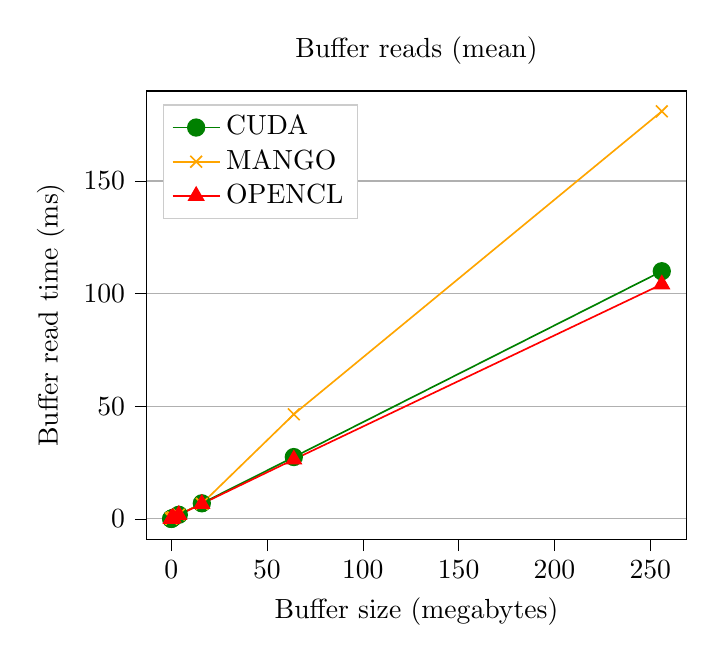
\begin{tikzpicture}

\definecolor{color0}{rgb}{1,0.647058823529412,0}

\begin{axis}[
legend cell align={left},
legend style={
  fill opacity=1,
  draw opacity=1,
  text opacity=1,
  at={(0.03,0.97)},
  anchor=north west,
  draw=white!80!black
},
tick align=outside,
tick pos=left,
title={Buffer reads (mean)},
x grid style={white!69.0196078431373!black},
xlabel={Buffer size (megabytes)},
xmin=-12.78359375, xmax=268.79921875,
xtick style={color=black},
y grid style={white!69.0196078431373!black},
ylabel={Buffer read time (ms)},
ymajorgrids,
ymin=-9.03422905142857, ymax=189.990061773878,
ytick style={color=black},
yticklabel style={/pgf/number format/fixed},
]
\addplot [semithick, green!50.1960784313725!black, mark=*, mark size=3, mark options={solid}]
table {%
0.015625 0.0123296224489796
0.0625 0.0205413469387755
0.25 0.130403275862069
1 0.505512620689655
4 1.83742425
16 6.9285274
64 27.4589087
256 109.953671
};
\addlegendentry{CUDA}
\addplot [semithick, color0, mark=x, mark size=3, mark options={solid}]
table {%
0.015625 0.0806020101010101
0.0625 0.16509962
0.25 0.282117206896552
1 0.732995033333333
4 1.89954115
16 6.7418782
64 46.451228
256 180.9435031
};
\addlegendentry{MANGO}
\addplot [semithick, red, mark=triangle*, mark size=3, mark options={solid}]
table {%
0.015625 0.0137764387755102
0.0625 0.02193194
0.25 0.136782633333333
1 0.511125655172414
4 1.78901245
16 6.68551331578947
64 26.398961
256 104.1510284
};
\addlegendentry{OPENCL}
\end{axis}

\end{tikzpicture}

        } 
    }}%
    \captionsetup{justification=centering}
    \caption{Mean buffer transfer times for HotSpot}%
    \label{fig:hotspot_buffer_transfers_mean}%
\end{figure}

\subsubsection{PathFinder}

Moving on to PathFinder we can see a much more significant difference in the performance of MANGO with respect to CUDA and OpenCL in figure \ref{fig:pathfinder_total_duration_mean}. Note that in PathFinder the number of kernel executions rises along with the input size, particularly the number of rows to process. A steeper rise in the execution time for MANGO indicates that the kernel execution overhead is piling up with the increased number of launches. 

\begin{figure}[ht]
    \centering
    \resizebox{0.6\textwidth}{!}{
        % This file was created by tikzplotlib v0.9.8.
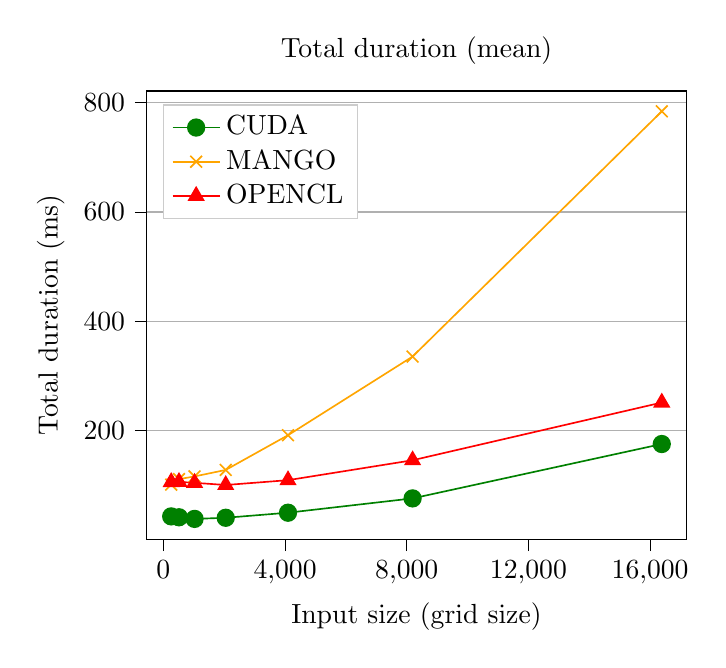
\begin{tikzpicture}

\definecolor{color0}{rgb}{1,0.647058823529412,0}

\begin{axis}[
legend cell align={left},
legend style={
  fill opacity=1,
  draw opacity=1,
  text opacity=1,
  at={(0.03,0.97)},
  anchor=north west,
  draw=white!80!black
},
tick align=outside,
tick pos=left,
title={Total duration (mean)},
x grid style={white!69.0196078431373!black},
xlabel={Input size (grid size)},
xmin=-550.4, xmax=17190.4,
xtick style={color=black},
y grid style={white!69.0196078431373!black},
ylabel={Total duration (ms)},
ymajorgrids,
ymin=1.06305218103449, ymax=821.428003991379,
ytick style={color=black},
scaled x ticks = false,
xtick={0, 4000, 8000, 12000, 16000},
]
\addplot [semithick, green!50.1960784313725!black, mark=*, mark size=3, mark options={solid}]
table {%
256 42.9552711
512 41.32715138
1024 38.3523681724138
2048 40.43792255
4096 49.69510795
8192 75.8983512
16384 175.3781874
};
\addlegendentry{CUDA}
\addplot [semithick, color0, mark=x, mark size=3, mark options={solid}]
table {%
256 101.184211525253
512 111.13555734
1024 116.082388233333
2048 127.939228894737
4096 191.4835014
8192 335.4150991
16384 784.138688
};
\addlegendentry{MANGO}
\addplot [semithick, red, mark=triangle*, mark size=3, mark options={solid}]
table {%
256 105.803828572917
512 106.067160145833
1024 104.400873965517
2048 100.396111
4096 109.2311212
8192 145.6926093
16384 251.2904586
};
\addlegendentry{OPENCL}
\end{axis}

\end{tikzpicture}

    }
    \captionsetup{justification=centering}
    \caption{Mean total execution time for PathFinder}
    \label{fig:pathfinder_total_duration_mean}
\end{figure}

In figure \ref{fig:pathfinder_kernel_execution_times} we can see that this kernel execution overhead fairly stable across the different input sizes, except for the initial benchmarks which have a very small size. In order to see the results more clearly and eliminate this fluctuation in the mean, we also included the minimum kernel execution times.

\begin{figure}[ht]%
    \centering
    \subfloat[\centering Mean kernel execution time]{{
        \resizebox{0.45\textwidth}{!}{
        % This file was created by tikzplotlib v0.9.8.
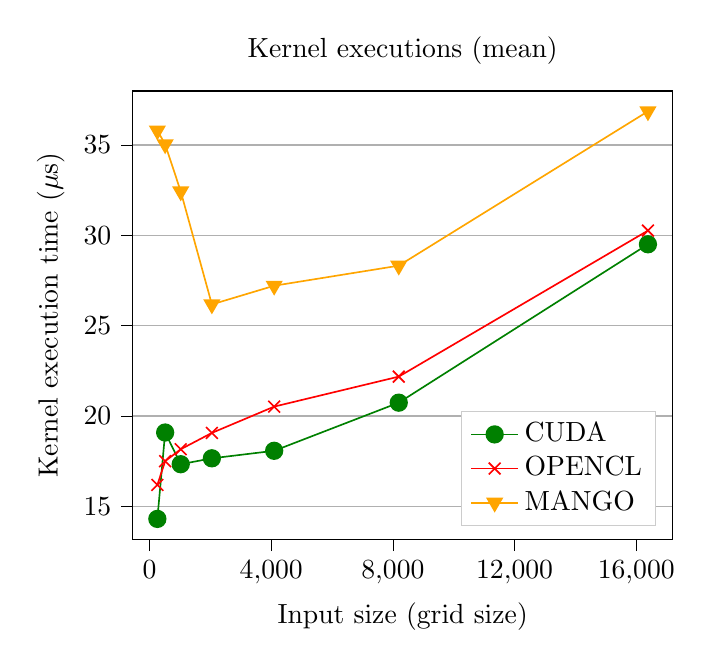
\begin{tikzpicture}

\definecolor{color0}{rgb}{1,0.647058823529412,0}

\begin{axis}[
legend cell align={left},
legend style={
  fill opacity=1,
  draw opacity=1,
  text opacity=1,
  at={(0.97,0.03)},
  anchor=south east,
  draw=white!80!black
},
tick align=outside,
tick pos=left,
title={Kernel executions (mean)},
x grid style={white!69.0196078431373!black},
xlabel={Input size (grid size)},
xmin=-550.4, xmax=17190.4,
xtick style={color=black},
y grid style={white!69.0196078431373!black},
ylabel={Kernel execution time ($\mu$s)},
ymajorgrids,
ymin=13.1755189830914, ymax=37.9917063550803,
ytick style={color=black},
scaled x ticks = false,
xtick={0, 4000, 8000, 12000, 16000},
]
\addplot [semithick, green!50.1960784313725!black, mark=*, mark size=3, mark options={solid}]
table {%
256 14.3035275
512 19.0845953667954
1024 17.3306496732026
2048 17.656685966634
4096 18.0730500490677
8192 20.7366837857667
16384 29.5047277512547
};
\addlegendentry{CUDA}
\addplot [semithick, red, mark=x, mark size=3, mark options={solid}]
table {%
256 16.1839365700861
512 17.4985770416025
1024 18.1579511051574
2048 19.0632247081712
4096 20.5183282178218
8192 22.1790555555556
16384 30.2621266070773
};
\addlegendentry{OPENCL}
\addplot [semithick, color0, mark=triangle*, mark size=3, mark options={solid,rotate=180}]
table {%
256 35.8026210691824
512 35.0376165354331
1024 32.4320626649077
2048 26.175443620178
4096 27.2096125186289
8192 28.3202890760466
16384 36.8636978381717
};
\addlegendentry{MANGO}
\end{axis}

\end{tikzpicture}

    } 
    }}%
    \qquad
    \subfloat[\centering Min kernel execution time]{{
        \resizebox{0.45\textwidth}{!}{
            % This file was created by tikzplotlib v0.9.8.
\begin{tikzpicture}

\definecolor{color0}{rgb}{1,0.647058823529412,0}

\begin{axis}[
legend cell align={left},
legend style={fill opacity=1, draw opacity=1, text opacity=1, draw=white!80!black},
tick align=outside,
tick pos=left,
title={Kernel executions (min)},
x grid style={white!69.0196078431373!black},
xlabel={Input size (grid size)},
xmin=-550.4, xmax=17190.4,
xtick style={color=black},
y grid style={white!69.0196078431373!black},
ylabel={Kernel execution time (μs)},
ymajorgrids,
ymin=6.1825, ymax=17.8095,
ytick style={color=black},
scaled x ticks = false,
xtick={0, 4000, 8000, 12000, 16000},
]
\addplot [semithick, green!50.1960784313725!black, mark=*, mark size=3, mark options={solid}]
table {%
256 11.924
512 10.761
1024 6.711
2048 9.254
4096 14.497
8192 13.4
16384 8.626
};
\addlegendentry{CUDA}
\addplot [semithick, red, mark=x, mark size=3, mark options={solid}]
table {%
256 12.901
512 11.82
1024 7.888
2048 10.449
4096 15.589
8192 14.153
16384 9.771
};
\addlegendentry{OPENCL}
\addplot [semithick, color0, mark=triangle*, mark size=3, mark options={solid,rotate=180}]
table {%
256 13.083
512 13.299
1024 9.495
2048 11.673
4096 17.281
8192 16.436
16384 11.432
};
\addlegendentry{MANGO}
\end{axis}

\end{tikzpicture}

        } 
    }}%
    \captionsetup{justification=centering}
    \caption{Kernel execution times for PathFinder}%
    \label{fig:pathfinder_kernel_execution_times}%
\end{figure}

Buffer transfers show a very similar story to HotSpot, with MANGO transfer times increasing at a much faster pace when compared with the other two models. PathFinder read times show much more variability than previous results, but this is largely based on the output of the kernel being much smaller than HotSpot's which increases the effect of any small but highly variable overhead. 

\begin{figure}[ht]%
    \centering
    \subfloat[\centering Mean buffer write time]{{
        \resizebox{0.45\textwidth}{!}{
        % This file was created by tikzplotlib v0.9.8.
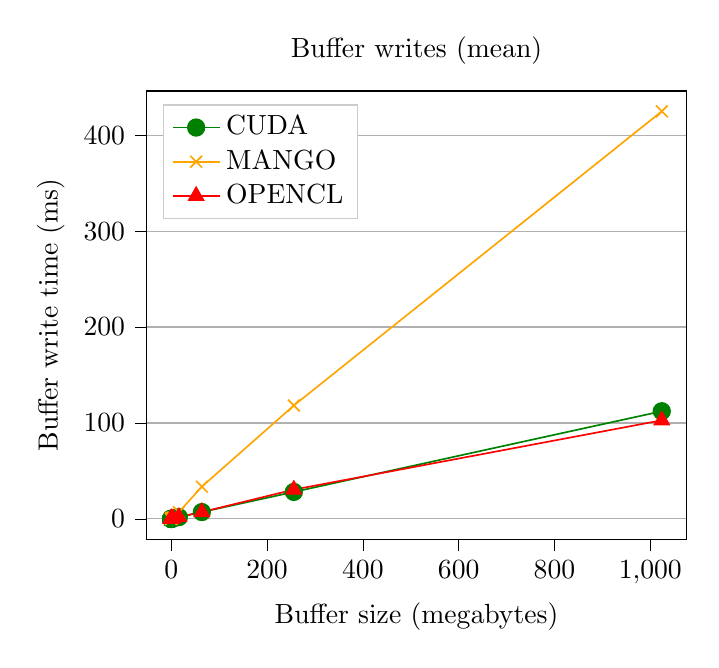
\begin{tikzpicture}

\definecolor{color0}{rgb}{1,0.647058823529412,0}

\begin{axis}[
legend cell align={left},
legend style={
  fill opacity=1,
  draw opacity=1,
  text opacity=1,
  at={(0.03,0.97)},
  anchor=north west,
  draw=white!80!black
},
tick align=outside,
tick pos=left,
title={Buffer writes (mean)},
x grid style={white!69.0196078431373!black},
xlabel={Buffer size (megabytes)},
xmin=-51.195849609375, xmax=1075.13432617188,
xtick style={color=black},
y grid style={white!69.0196078431373!black},
ylabel={Buffer write time (ms)},
ymajorgrids,
ymin=-21.2301063907143, ymax=446.080604551939,
ytick style={color=black},
yticklabel style={/pgf/number format/fixed},
]
\addplot [semithick, green!50.1960784313725!black, mark=*, mark size=3, mark options={solid}]
table {%
0.0009765625 0.0112895612244898
0.001953125 0.01208368
0.00390625 0.0117242333333333
0.0078125 0.0129084736842105
0.015625 0.01453375
0.03125 0.0176991
0.0625 0.0208775
0.2490234375 0.0286712755102041
0.998046875 0.10126693877551
3.99609375 0.459110655172414
15.9921875 1.80984045
63.984375 7.13521621052632
255.96875 28.1117542
1023.9375 112.2217462
};
\addlegendentry{CUDA}
\addplot [semithick, color0, mark=x, mark size=3, mark options={solid}]
table {%
0.0009765625 0.17391198989899
0.001953125 0.17851804
0.00390625 0.165922633333333
0.0078125 0.1528704
0.015625 0.1705615
0.03125 0.1738537
0.0625 0.7945439
0.2490234375 0.300501707070707
0.998046875 0.60951162
3.99609375 1.45868382758621
15.9921875 7.00193921052632
63.984375 33.6318241
255.96875 118.210402
1023.9375 424.8392086
};
\addlegendentry{MANGO}
\addplot [semithick, red, mark=triangle*, mark size=3, mark options={solid}]
table {%
0.0009765625 0.21893114
0.001953125 0.21817348
0.00390625 0.226192172413793
0.0078125 0.22287355
0.015625 0.2213049
0.03125 0.2202647
0.0625 0.2337682
0.2490234375 0.0643956597938144
0.998046875 0.19593170212766
3.99609375 0.621945551724138
15.9921875 1.96354655
63.984375 7.15548315
255.96875 30.5490241
1023.9375 102.7730812
};
\addlegendentry{OPENCL}
\end{axis}

\end{tikzpicture}

    } 
    }}%
    \qquad
    \subfloat[\centering Mean buffer read time]{{
        \resizebox{0.45\textwidth}{!}{
            % This file was created by tikzplotlib v0.9.8.
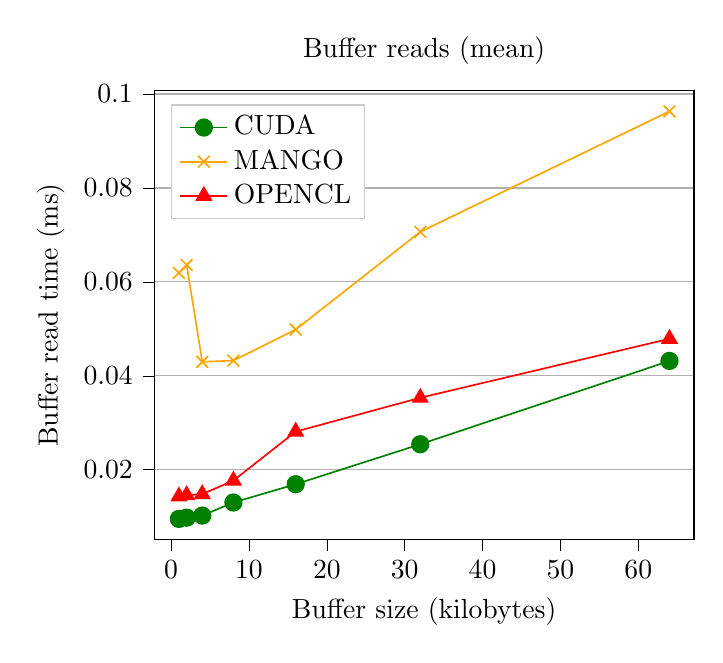
\begin{tikzpicture}

\definecolor{color0}{rgb}{1,0.647058823529412,0}

\begin{axis}[
legend cell align={left},
legend style={
  fill opacity=1,
  draw opacity=1,
  text opacity=1,
  at={(0.03,0.97)},
  anchor=north west,
  draw=white!80!black
},
tick align=outside,
tick pos=left,
title={Buffer reads (mean)},
x grid style={white!69.0196078431373!black},
xlabel={Buffer size (kilobytes)},
xmin=-2.15, xmax=67.15,
xtick style={color=black},
y grid style={white!69.0196078431373!black},
ylabel={Buffer read time (ms)},
ymajorgrids,
ymin=0.00520630214285714, ymax=0.100653614183673,
ytick style={color=black},
yticklabel style={/pgf/number format/fixed},
]
\addplot [semithick, green!50.1960784313725!black, mark=*, mark size=3, mark options={solid}]
table {%
1 0.00954481632653061
2 0.0097984693877551
4 0.0102500714285714
8 0.01303545
16 0.01692725
32 0.0254355
64 0.0431711
};
\addlegendentry{CUDA}
\addplot [semithick, color0, mark=x, mark size=3, mark options={solid}]
table {%
1 0.0619118
2 0.06359902
4 0.0429807333333333
8 0.0432455789473684
16 0.04984925
32 0.0706595
64 0.0963151
};
\addlegendentry{MANGO}
\addplot [semithick, red, mark=triangle*, mark size=3, mark options={solid}]
table {%
1 0.0143187777777778
2 0.01460112
4 0.0148169
8 0.01770105
16 0.02812495
32 0.0353335
64 0.0478901
};
\addlegendentry{OPENCL}
\end{axis}

\end{tikzpicture}

        } 
    }}%
    \captionsetup{justification=centering}
    \caption{Mean buffer transfer times for PathFinder}%
    \label{fig:pathfinder_buffer_transfers_mean}%
\end{figure}

\subsubsection{AXPY}

In AXPY we move straight to the mean kernel execution time in figure \ref{fig:axpy_kernel_executions_mean} where we can see that MANGO performs 24.5\% slower than CUDA and 17.4\% slower than OpenCL for the same size input.

\begin{figure}[ht]
    \centering
    \resizebox{0.6\textwidth}{!}{
        % This file was created by tikzplotlib v0.9.8.
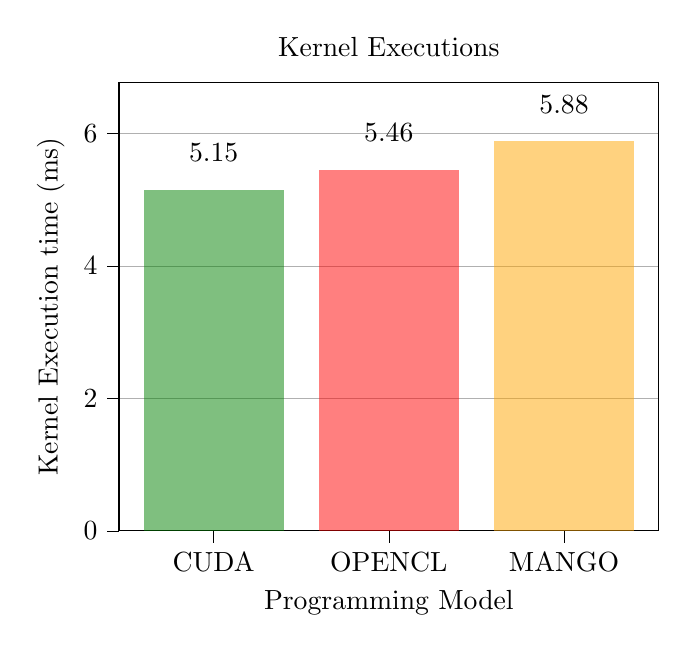
\begin{tikzpicture}

\definecolor{color0}{rgb}{1,0.647058823529412,0}

\begin{axis}[
tick align=outside,
tick pos=left,
title={Kernel Executions},
x grid style={white!69.0196078431373!black},
xlabel={Programming Model},
xmin=-0.54, xmax=2.54,
xtick style={color=black},
xtick={0,1,2},
xticklabels={CUDA,OPENCL,MANGO},
y grid style={white!69.0196078431373!black},
ylabel={Kernel Execution time (ms)},
ymajorgrids,
ymin=0, ymax=6.7738881661,
ytick style={color=black}
]
\draw[draw=none,fill=green!50.1960784313725!black,fill opacity=0.5] (axis cs:-0.4,0) rectangle (axis cs:0.4,5.15266011);
\draw[draw=none,fill=red,fill opacity=0.5] (axis cs:0.6,0) rectangle (axis cs:1.4,5.45583448);
\draw[draw=none,fill=color0,fill opacity=0.5] (axis cs:1.6,0) rectangle (axis cs:2.4,5.88321827);
\draw (axis cs:0,5.427521991) node[
  scale=1,
  anchor=south,
  text=black,
  rotate=0.0
]{5.15};
\draw (axis cs:1,5.730696361) node[
  scale=1,
  anchor=south,
  text=black,
  rotate=0.0
]{5.46};
\draw (axis cs:2,6.158080151) node[
  scale=1,
  anchor=south,
  text=black,
  rotate=0.0
]{5.88};
\end{axis}

\end{tikzpicture}

    }
    \captionsetup{justification=centering}
    \caption{Mean kernel execution times for AXPY}
    \label{fig:axpy_kernel_executions_mean}
\end{figure}

As we know that AXPY is purely memory bandwidth bound, we can translate this kernel execution times to memory bandwidth measurements as seen in figure \ref{fig:axpy_bandwidth_mean}. In this figure we can see the percentage of theoretical peak bandwidth achieved by each programming model.

\begin{figure}[ht]
    \centering
    \resizebox{0.6\textwidth}{!}{
        % This file was created by tikzplotlib v0.9.8.
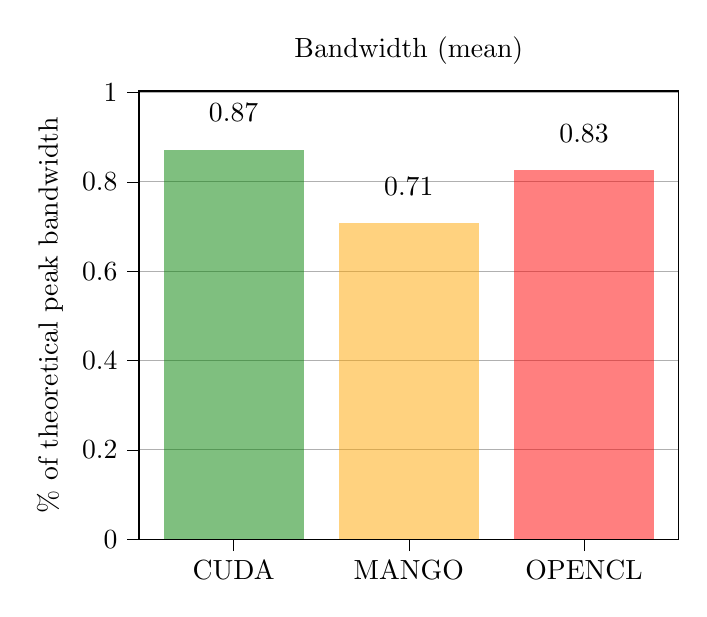
\begin{tikzpicture}

\definecolor{color0}{rgb}{1,0.647058823529412,0}

\begin{axis}[
tick align=outside,
tick pos=left,
title={Bandwidth (mean)},
x grid style={white!69.0196078431373!black},
xmin=-0.54, xmax=2.54,
xtick style={color=black},
xtick={0,1,2},
xticklabels={CUDA,MANGO,OPENCL},
y grid style={white!69.0196078431373!black},
ylabel={\% of theoretical peak bandwidth},
ymajorgrids,
ymin=0, ymax=1.00347644198507,
ytick style={color=black},
yticklabel style={/pgf/number format/fixed},
]
\draw[draw=none,fill=green!50.1960784313725!black,fill opacity=0.5] (axis cs:-0.4,0) rectangle (axis cs:0.4,0.872156563953115);
\draw[draw=none,fill=color0,fill opacity=0.5] (axis cs:0.6,0) rectangle (axis cs:1.4,0.707407075302276);
\draw[draw=none,fill=red,fill opacity=0.5] (axis cs:1.6,0) rectangle (axis cs:2.4,0.826121177288947);
\draw (axis cs:0,0.91225131089552) node[
  scale=1,
  anchor=south,
  text=black,
  rotate=0.0
]{0.87};
\draw (axis cs:1,0.747501822244682) node[
  scale=1,
  anchor=south,
  text=black,
  rotate=0.0
]{0.71};
\draw (axis cs:2,0.866215924231353) node[
  scale=1,
  anchor=south,
  text=black,
  rotate=0.0
]{0.83};
\end{axis}

\end{tikzpicture}

    }
    \captionsetup{justification=centering}
    \caption{Mean GPU memory bandwidth for AXPY}
    \label{fig:axpy_bandwidth_mean}
\end{figure}

What is interesting is that if we look at the maximum bandwidth achieved by each model MANGO is able to tie OpenCL, being just 3\% less bandwidth efficient than pure CUDA code. 

\begin{figure}[ht]
    \centering
    \resizebox{0.6\textwidth}{!}{
        % This file was created by tikzplotlib v0.9.8.
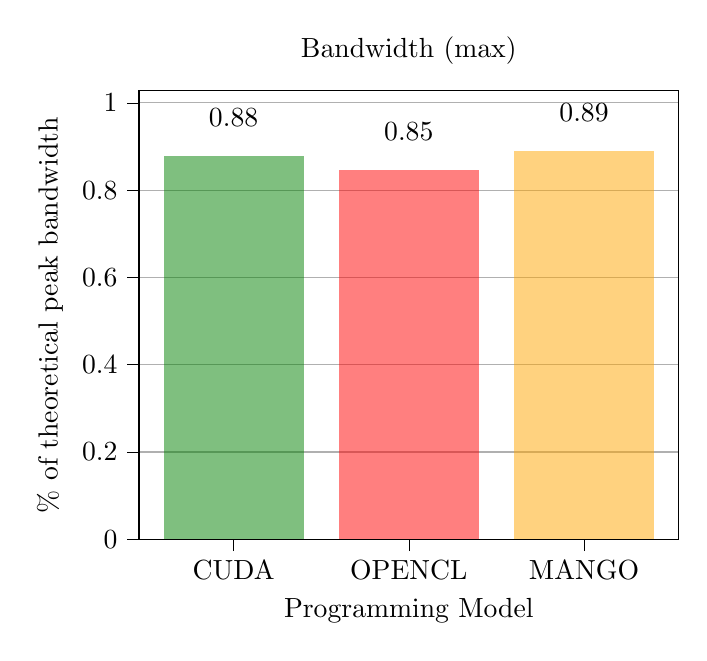
\begin{tikzpicture}

\definecolor{color0}{rgb}{1,0.647058823529412,0}

\begin{axis}[
tick align=outside,
tick pos=left,
title={Bandwidth (max)},
x grid style={white!69.0196078431373!black},
xlabel={Programming Model},
xmin=-0.54, xmax=2.54,
xtick style={color=black},
xtick={0,1,2},
xticklabels={CUDA,OPENCL,MANGO},
y grid style={white!69.0196078431373!black},
ylabel={\% of theoretical peak bandwidth},
ymajorgrids,
ymin=0, ymax=1.02734953480631,
ytick style={color=black}
]
\draw[draw=none,fill=green!50.1960784313725!black,fill opacity=0.5] (axis cs:-0.4,0) rectangle (axis cs:0.4,0.87937553130392);
\draw[draw=none,fill=red,fill opacity=0.5] (axis cs:0.6,0) rectangle (axis cs:1.4,0.846996642648818);
\draw[draw=none,fill=color0,fill opacity=0.5] (axis cs:1.6,0) rectangle (axis cs:2.4,0.890342216051125);
\draw (axis cs:0,0.922987437803984) node[
  scale=1,
  anchor=south,
  text=black,
  rotate=0.0
]{0.88};
\draw (axis cs:1,0.890608549148883) node[
  scale=1,
  anchor=south,
  text=black,
  rotate=0.0
]{0.85};
\draw (axis cs:2,0.933954122551189) node[
  scale=1,
  anchor=south,
  text=black,
  rotate=0.0
]{0.89};
\end{axis}

\end{tikzpicture}

    }
    \captionsetup{justification=centering}
    \caption{Max GPU memory bandwidth for AXPY}
    \label{fig:axpy_bandwidth_max}
\end{figure}

Finally, we look at the transfer times achieved between the host and the device and vice versa and how these translate to the percentage of PCI-E bandwidth achieved. These comparisons can be seen in figures \ref{fig:axpy_buffer_transfers_mean} and \ref{fig:axpy_buffer_transfers_bandwidth_mean} respectively. Here the difference between MANGO and the other models is considerable. For host to device transfers, our MANGO implementation manages to be almost three times slower than CUDA and OpenCL, and almost twice as slow for device to host transfers.

\begin{figure}[ht]%
    \centering
    \subfloat[\centering Mean buffer write time]{{
        \resizebox{0.45\textwidth}{!}{
        % This file was created by tikzplotlib v0.9.8.
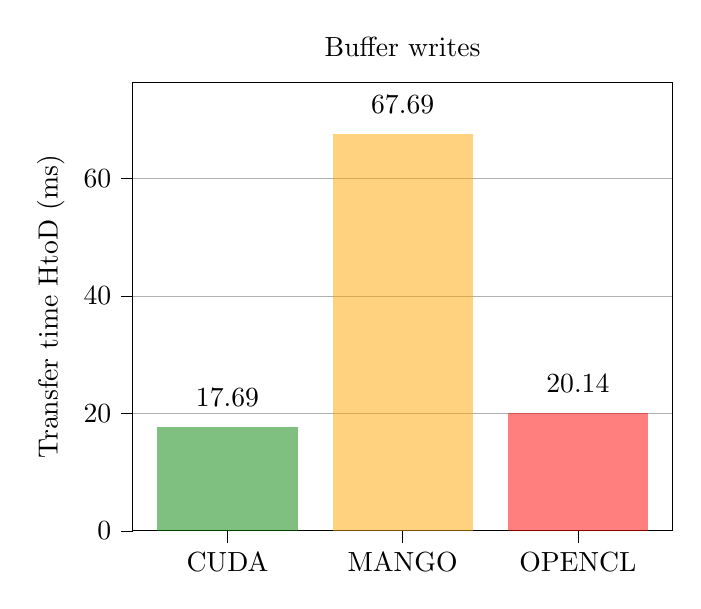
\begin{tikzpicture}

\definecolor{color0}{rgb}{1,0.647058823529412,0}

\begin{axis}[
tick align=outside,
tick pos=left,
title={Buffer writes},
x grid style={white!69.0196078431373!black},
xmin=-0.54, xmax=2.54,
xtick style={color=black},
xtick={0,1,2},
xticklabels={CUDA,MANGO,OPENCL},
y grid style={white!69.0196078431373!black},
ylabel={Transfer time HtoD (ms)},
ymajorgrids,
ymin=0, ymax=76.3910404992625,
ytick style={color=black},
yticklabel style={/pgf/number format/fixed},
]
\draw[draw=none,fill=green!50.1960784313725!black,fill opacity=0.5] (axis cs:-0.4,0) rectangle (axis cs:0.4,17.68977225);
\draw[draw=none,fill=color0,fill opacity=0.5] (axis cs:0.6,0) rectangle (axis cs:1.4,67.6877919275);
\draw[draw=none,fill=red,fill opacity=0.5] (axis cs:1.6,0) rectangle (axis cs:2.4,20.138947405);
\draw (axis cs:0,19.448380776375) node[
  scale=1,
  anchor=south,
  text=black,
  rotate=0.0
]{17.69};
\draw (axis cs:1,69.446400453875) node[
  scale=1,
  anchor=south,
  text=black,
  rotate=0.0
]{67.69};
\draw (axis cs:2,21.897555931375) node[
  scale=1,
  anchor=south,
  text=black,
  rotate=0.0
]{20.14};
\end{axis}

\end{tikzpicture}

    } 
    }}%
    \qquad
    \subfloat[\centering Mean buffer read time]{{
        \resizebox{0.45\textwidth}{!}{
            % This file was created by tikzplotlib v0.9.8.
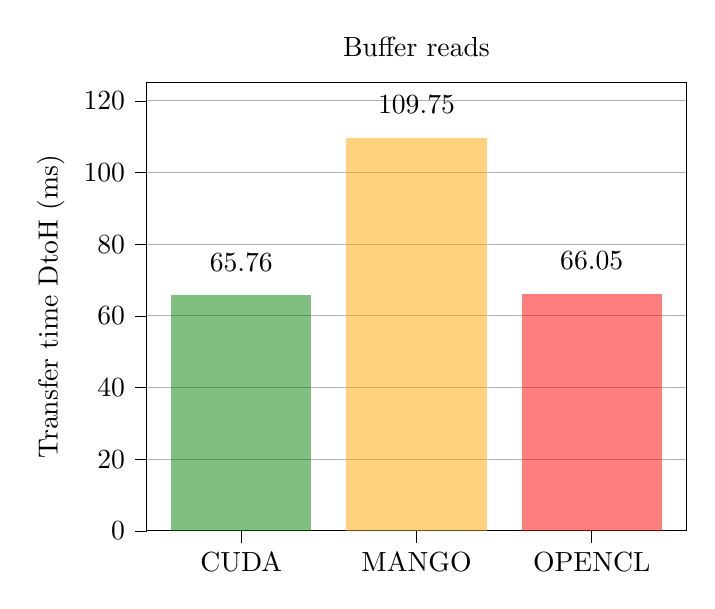
\begin{tikzpicture}

\definecolor{color0}{rgb}{1,0.647058823529412,0}

\begin{axis}[
tick align=outside,
tick pos=left,
title={Buffer reads},
x grid style={white!69.0196078431373!black},
xmin=-0.54, xmax=2.54,
xtick style={color=black},
xtick={0,1,2},
xticklabels={CUDA,MANGO,OPENCL},
y grid style={white!69.0196078431373!black},
ylabel={Transfer time DtoH (ms)},
ymajorgrids,
ymin=0, ymax=125.150330663325,
ytick style={color=black},
yticklabel style={/pgf/number format/fixed},
]
\draw[draw=none,fill=green!50.1960784313725!black,fill opacity=0.5] (axis cs:-0.4,0) rectangle (axis cs:0.4,65.76414157);
\draw[draw=none,fill=color0,fill opacity=0.5] (axis cs:0.6,0) rectangle (axis cs:1.4,109.746946745);
\draw[draw=none,fill=red,fill opacity=0.5] (axis cs:1.6,0) rectangle (axis cs:2.4,66.05377953);
\draw (axis cs:0,69.79022270075) node[
  scale=1,
  anchor=south,
  text=black,
  rotate=0.0
]{65.76};
\draw (axis cs:1,113.77302787575) node[
  scale=1,
  anchor=south,
  text=black,
  rotate=0.0
]{109.75};
\draw (axis cs:2,70.07986066075) node[
  scale=1,
  anchor=south,
  text=black,
  rotate=0.0
]{66.05};
\end{axis}

\end{tikzpicture}

        } 
    }}%
    \captionsetup{justification=centering}
    \caption{Mean buffer transfer times for AXPY}%
    \label{fig:axpy_buffer_transfers_mean}%
\end{figure}

\begin{figure}[ht]%
    \centering
    \subfloat[\centering Mean host to device transfer bandwidth]{{
        \resizebox{0.45\textwidth}{!}{
        % This file was created by tikzplotlib v0.9.8.
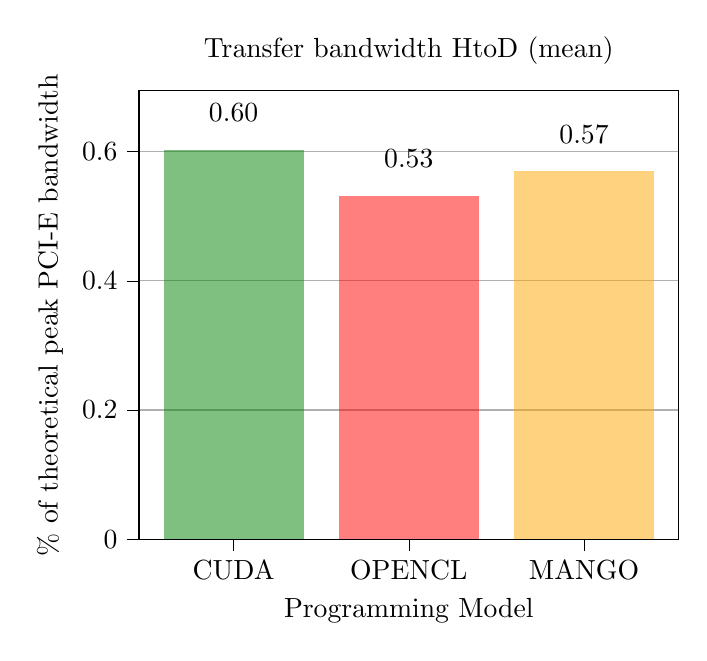
\begin{tikzpicture}

\definecolor{color0}{rgb}{1,0.647058823529412,0}

\begin{axis}[
tick align=outside,
tick pos=left,
title={Transfer bandwidth HtoD (mean)},
x grid style={white!69.0196078431373!black},
xlabel={Programming Model},
xmin=-0.54, xmax=2.54,
xtick style={color=black},
xtick={0,1,2},
xticklabels={CUDA,OPENCL,MANGO},
y grid style={white!69.0196078431373!black},
ylabel={\% of theoretical peak PCI-E bandwidth},
ymajorgrids,
ymin=0, ymax=0.693817866752193,
ytick style={color=black}
]
\draw[draw=none,fill=green!50.1960784313725!black,fill opacity=0.5] (axis cs:-0.4,0) rectangle (axis cs:0.4,0.602361171863845);
\draw[draw=none,fill=red,fill opacity=0.5] (axis cs:0.6,0) rectangle (axis cs:1.4,0.53135754934798);
\draw[draw=none,fill=color0,fill opacity=0.5] (axis cs:1.6,0) rectangle (axis cs:2.4,0.569221880713467);
\draw (axis cs:0,0.630743515229267) node[
  scale=1,
  anchor=south,
  text=black,
  rotate=0.0
]{0.60};
\draw (axis cs:1,0.559739892713401) node[
  scale=1,
  anchor=south,
  text=black,
  rotate=0.0
]{0.53};
\draw (axis cs:2,0.597604224078889) node[
  scale=1,
  anchor=south,
  text=black,
  rotate=0.0
]{0.57};
\end{axis}

\end{tikzpicture}

    } 
    }}%
    \qquad
    \subfloat[\centering Mean device to host transfer bandwidth]{{
        \resizebox{0.45\textwidth}{!}{
            % This file was created by tikzplotlib v0.9.8.
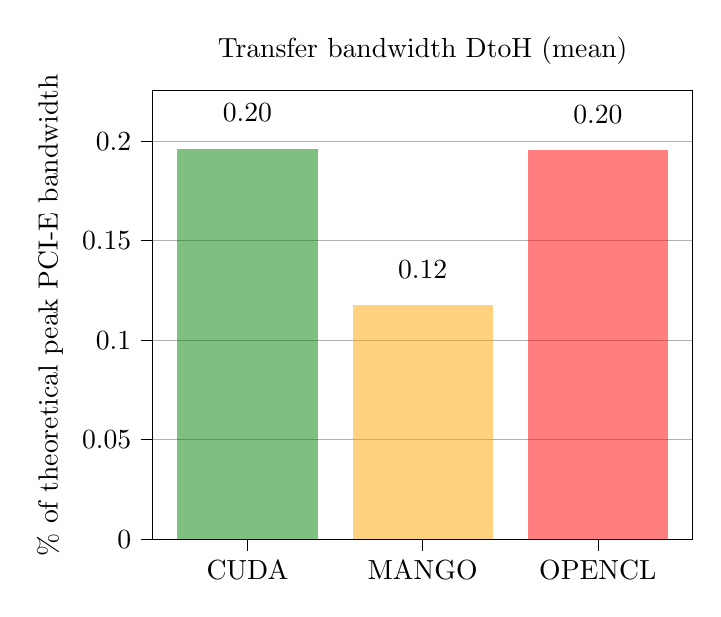
\begin{tikzpicture}

\definecolor{color0}{rgb}{1,0.647058823529412,0}

\begin{axis}[
tick align=outside,
tick pos=left,
title={Transfer bandwidth DtoH (mean)},
x grid style={white!69.0196078431373!black},
xmin=-0.54, xmax=2.54,
xtick style={color=black},
xtick={0,1,2},
xticklabels={CUDA,MANGO,OPENCL},
y grid style={white!69.0196078431373!black},
ylabel={\% of theoretical peak PCI-E bandwidth},
ymajorgrids,
ymin=0, ymax=0.225207888741475,
ytick style={color=black},
yticklabel style={/pgf/number format/fixed},
]
\draw[draw=none,fill=green!50.1960784313725!black,fill opacity=0.5] (axis cs:-0.4,0) rectangle (axis cs:0.4,0.196246840753961);
\draw[draw=none,fill=color0,fill opacity=0.5] (axis cs:0.6,0) rectangle (axis cs:1.4,0.11760810305661);
\draw[draw=none,fill=red,fill opacity=0.5] (axis cs:1.6,0) rectangle (axis cs:2.4,0.195401269577688);
\draw (axis cs:0,0.204734444310432) node[
  scale=1,
  anchor=south,
  text=black,
  rotate=0.0
]{0.20};
\draw (axis cs:1,0.126095706613081) node[
  scale=1,
  anchor=south,
  text=black,
  rotate=0.0
]{0.12};
\draw (axis cs:2,0.203888873134159) node[
  scale=1,
  anchor=south,
  text=black,
  rotate=0.0
]{0.20};
\end{axis}

\end{tikzpicture}

        } 
    }}%
    \captionsetup{justification=centering}
    \caption{Mean buffer transfer times for AXPY}%
    \label{fig:axpy_buffer_transfers_bandwidth_mean}%
\end{figure}

\subsubsection{Overall Analysis}

Our initial implementation of the HHAL and restructuring of the MANGO stack is certainly not competitive with state-of-the-art programming models such as CUDA and OpenCL. 

Both kernel execution and buffer transfer overheads can be linked with our client-server approach when integrating the HHAL with the rest of the software. 

Both Barbeque and MANGO need access to the HHAL for different reasons. Barbeque needs to allocate and deallocate resources and MANGO needs to execute the kernels. As barbeque and MANGO do not co-exist in the same process (Barbeque always works as a daemon) and there is this need to give both access to the same HHAL information we moved the HHAL to its own process. This works without any problems to communicate information and maintain a consistent state across all processes. 

However, as the entirety of the HHAL is behind a central server with a socket based connection to the different clients, this means that both kernel launches and buffer transfers need to go through the socket first.

Relying on inter-process communication (IPC) for all operations significantly decreases the performance that can be achieved by MANGO, specially when using sockets over a much more efficient alternative like shared memory.

During our development of the HHAL, our main focus was to improve the extensibility of the MANGO platform by decoupling it from the HN library, thus providing a more general internal API for communicating with each available architecture. In consequence, we opted for a faster development approach and oversaw the performance implications of excessive and inefficient IPC.

Although for proper decoupling of the MANGO library from architectural changes it is necessary for at least part of the HHAL to continue existing as a separate process. Nonetheless, the HHAL API could be split to allow for the performance critical aspects of the code to be executed directly in the client process, thus forgoing the need to, for example, transfer the entirety of the buffer data through a socket.

\subsection{Programmability}

The results for the HotSpot benchmark can be seen in table \ref{tab:hotspot-loc} while the ones for PathFinder are in table \ref{tab:pathfinder-loc}.

\begin{table}[ht]
    \centering
    \begin{tabular}{l|c|c|c|c|c|c}
    \textit{Model} & \textit{Kernel (LOC)} & \textit{Kernel (RD)} & \textit{Host (LOC)} & \textit{Host (RD)} & \textit{Total (LOC)} & \textit{Total (RD)} \\ \hline
    MANGO & 84 & 0\% & 190 & 0\% & 274 & 0\% \\
    CUDA & 84 & 0\% & 166 & -13\% & 250 & -9\% \\
    OpenCL & 84 & 0\% & 212 & 12\% & 296 & 8\%  
    \end{tabular}
    \captionsetup{justification=centering}
    \caption{Lines of code for HotSpot benchmark}
    \label{tab:hotspot-loc}
\end{table}

\begin{table}[ht]
    \centering
    \begin{tabular}{l|c|c|c|c|c|c}
    \textit{Model} & \textit{Kernel (LOC)} & \textit{Kernel (RD)} & \textit{Host (LOC)} & \textit{Host (RD)} & \textit{Total (LOC)} & \textit{Total (RD)} \\ \hline
    MANGO & 59 & 0\% & 133 & 0\% & 192 & 0\% \\
    CUDA & 59 & 0\% & 108 & -19\% & 167 & -13\% \\
    OpenCL & 59 & 0\% & 188 & 41\% & 247 & 29\%  
    \end{tabular}
    \captionsetup{justification=centering}
    \caption{Lines of code for PathFinder benchmark}
    \label{tab:pathfinder-loc}
\end{table}

When comparing kernel LOC we can see that they are equal across all implementations of the same benchmark. As MANGO uses the same kernel code as the CUDA implementation, this is expected. In the case of OpenCL, its kernels are also optimized for GPU execution and thus follow the same access pattern as a CUDA kernel. The only differences among the kernels being CUDA and OpenCL specific keywords and functions, which have a 1-to-1 mapping between each other.

On the host side, the CUDA implementation gains the upper hand on MANGO, needing 9\% less code for HotSpot and 13\% less code for PathFinder. On the other hand OpenCL requires 8\% and 29\% more code for each respective benchmark. These differences are mostly related to the following factors:

\textbf{Kernel function calls:} the single source nature of CUDA code allows these implementations to call a kernel like any other function. Meanwhile MANGO requires creating multiple argument objects, one for each of the kernel inputs and grouping them into a \texttt{KernelArguments} object to be able to start the kernel execution. OpenCL faces a similar issue as it also needs explicit \texttt{setKernelArg} calls for each kernel input. This gives a big advantage to CUDA, with MANGO and OpenCL being very similar to each other.

\textbf{Kernel loading:} both MANGO and OpenCL need to load kernel code from an external file. For MANGO this only requires creating a \texttt{KernelFunction} object, loading a file (single call to the \texttt{load} function of a \texttt{KernelFunction}) and registering the kernel to the \texttt{Context}. Meanwhile OpenCL requests that the kernel code is provided as a C string, leaving the file loading code to the user, who also needs to make function calls to build the program and create a kernel object. The CUDA implementation is not required to do any of the previous work, as the kernel code can be called directly and is compiled along with the host code.

\textbf{Resource deallocations:} while all programming models need to explicitly request resource allocation for input and output buffers, MANGO does not leave the user with the responsibility to perform the inverse operations, at least not individually. When the MANGO implementations finish, they can simply call the context deallocation function and all requested resources will be correctly released. On the other hand, both OpenCL and CUDA require explicit release of resources. In the case of CUDA, this only entails calling \texttt{cudaFree} for each \texttt{cudaMalloc} call, for OpenCL it is much more involved, however. The programmer needs to release, on top of the allocated buffers, the following resources: \texttt{CommandQueue}, \texttt{Kernel}, \texttt{Program}, \texttt{Context}, a buffer for the program source string, a buffer for querying device ids and a buffer for querying platform ids.

\textbf{Device selection:} OpenCL requires manual querying of the available platforms on the host as well as the available devices in order to select the device to use for the benchmark. Both are multi-step processes requiring multiple function calls and host heap memory allocations. As CUDA only runs on NVIDIA GPUs, one only needs to select a particular device ID among the ones available, but that can also be skipped (and was, for our tests) if there is only a single GPU available or there is no preference in which GPU to run the kernel. Finally, MANGO does all this work automatically, needing no input from the user apart from providing the device kernels along with information about which platform they target (in this case NVIDIA). In the background, BBQUE and the HHAL will make sure to assign the kernel to run on the most suitable device.

\textbf{Error handling:} as both CUDA and OpenCL work with exit codes in order to communicate runtime errors, there is a need to perform explicit error handling at each function call in their benchmark implementations. For brevity, most of this error handling was extracted into preprocessor macros, so they do not contribute significantly to the total LOC. Some OpenCL calls however cannot be easily handled by a macro and need extra error handling code. Meanwhile, the last layer of the MANGO API maps runtime errors into exceptions so they can be handled more easily by the user.

A breakdown of LOC differences for these particular sections of the code in both benchmarks can be seen in tables \ref{tab:hotspot-factors-loc} and \ref{tab:pathfinder-factors-loc} which refer to HotSpot and PathFinder respectively. As shown here, the main disadvantage of MANGO over CUDA is due to the kernel call code. This could be improved by leveraging C++'s templates, allowing for a variety of argument types and quantities to be supplied directly to MANGO's \texttt{kernel\_launch} call. This will turn the implementation of the function significantly more complex, but will provide a much more concise API for the users of the platform.

\begin{table}[ht]
    \centering
    \begin{tabular}{l|c|c|c|c|c|c}
    \textit{Model} & \textit{Kernel call} & \textit{Kernel load} & \textit{Deallocations} & \textit{Device select} & \textit{Error handling} & \textit{Total} \\ \hline
    MANGO & 20 & 3 & 1 & 0 & 0 & 24 \\
    CUDA & 7 & 0 & 3 & 0 & 7 & 17 \\
    OpenCL & 16 & 16 & 10 & 14 & 14 & 70  
    \end{tabular}
    \captionsetup{justification=centering}
    \caption{Size of relevant sections of code in HotSpot benchmark}
    \label{tab:hotspot-factors-loc}
\end{table}

\begin{table}[ht]
    \centering
    \begin{tabular}{l|c|c|c|c|c|c}
    \textit{Model} & \textit{Kernel call} & \textit{Kernel load} & \textit{Deallocations} & \textit{Device select} & \textit{Error handling} & \textit{Total} \\ \hline
    MANGO & 15 & 3 & 1 & 0 & 0 & 19 \\
    CUDA & 6 & 0 & 3 & 0 & 7 & 16 \\
    OpenCL & 11 & 16 & 10 & 14 & 14 & 65  
    \end{tabular}
    \captionsetup{justification=centering}
    \caption{Size of relevant sections of code in PathFinder benchmark}
    \label{tab:pathfinder-factors-loc}
\end{table}

